% =====================================================================
% Microfluidics and Nanofluidics (Springer Nature) research article
% =====================================================================
% TARGET JOURNAL: Microfluidics and Nanofluidics (Springer Nature).
% REFERENCE STYLE: sn-basic (Springer Nature basic AUTHOR-YEAR style).
%   Microfluidics and Nanofluidics uses author-year in-text citations,
%   "(Author Year)" / "Author (Year)" via natbib \citep / \citet.
% COMPILE INSTRUCTIONS:
%   Compile this file with the official Springer Nature unified LaTeX
%   (sn-jnl) bundle. The class file sn-jnl.cls and the bibliography style
%   bst/sn-basic.bst are provided alongside this file in paper/. To build:
%     1. Keep sn-jnl.cls and bst/sn-basic.bst alongside this .tex file
%        (they are already in paper/).
%     2. Add references.bib and the figures/ directory to the project.
%     3. Compile with pdfLaTeX -> BibTeX -> pdfLaTeX x2.
%   The \documentclass option sn-basic selects the author-year .bst, so
%   \bibliography{references} needs no further style declaration.
% =====================================================================
\documentclass[pdflatex,sn-basic]{sn-jnl}

\usepackage{graphicx}
\usepackage{multirow}
\usepackage{amsmath,amssymb,amsfonts}
\usepackage{amsthm}
\usepackage{mathrsfs}
\usepackage[title]{appendix}
\usepackage{xcolor}
\usepackage{textcomp}
\usepackage{manyfoot}
\usepackage{booktabs}
\usepackage{algorithm}
\usepackage{algorithmicx}
\usepackage{algpseudocode}
\usepackage{listings}
\usepackage{url}
\usepackage{siunitx}
\sisetup{
  per-mode=symbol,
  inter-unit-product=\ensuremath{\cdot},
  range-phrase=--,
  range-units=single
}
\DeclareSIUnit\decibel{dB}
\DeclareSIUnit\minute{min}
\DeclareSIUnit\hour{h}
\DeclareSIUnit\day{d}

\theoremstyle{thmstyleone}
\newtheorem{theorem}{Theorem}
\newtheorem{proposition}[theorem]{Proposition}
\newtheorem{example}{Example}
\newtheorem{remark}{Remark}
\theoremstyle{thmstyletwo}
\newtheorem{definition}{Definition}
\theoremstyle{thmstylethree}
\newtheorem{note}{Note}

\raggedbottom

% =====================================================================
\begin{document}

% ---------------------------------------------------------------------
% SUBMISSION NOTE (Microfluidics and Nanofluidics):
%   M&N does not require a separate graphical abstract. For the technical
%   check, upload this .tex with the figures (and the sn-jnl.cls + sn-basic
%   .bst + references.bib needed to compile) in a single zip; the publisher
%   compiles it to a review PDF. Initial submission is otherwise a PDF.
% ---------------------------------------------------------------------

\title[$\mu$Flow: an interactive simulator for microfluidic Hall-effect bead detection]{$\mu$Flow: An Interactive Simulator for Microfluidic Hall-Effect Magnetic Bead Detection with Parametric Design Optimization}

\author*[1]{\fnm{Harshitha} \sur{Govindaraju}}\email{harshitha.govindaraju@rutgers.edu}

\author[1]{\fnm{Umer} \sur{Hassan}}\email{umer.hassan@rutgers.edu}

\affil[1]{\orgdiv{Department of Electrical and Computer Engineering}, \orgname{Rutgers, The State University of New Jersey}, \orgaddress{\street{94 Brett Road}, \city{Piscataway}, \state{NJ}, \postcode{08854}, \country{USA}}}

% ORCID: Microfluidics and Nanofluidics requests the full 16-digit ORCID for each
% author on the title page. In this sn-jnl bundle, \orcid{<full ORCID URL>}
% renders the ORCID logo as a hyperlink but also requires the Orcidlogo.eps
% asset (not shipped here), so it is intentionally not invoked above.
% TODO before submission: insert each author's real 16-digit ORCID on the
% title page (e.g. as \orcid{https://orcid.org/0000-0000-0000-0000} once the
% Orcidlogo.eps asset from the official template is added, or via the
% submission-system author metadata). Do NOT use a placeholder ID at submission.

\abstract{$\mu$Flow is an interactive, browser-based simulator for microfluidic Hall-effect detection of superparamagnetic beads, built for parametric design optimization of the sensor before fabrication. It couples a closed-form model of the full signal chain: Clausius--Mossotti bead magnetization with a volume-fraction correction, a point-dipole stray field, a volume-averaged Hall voltage with geometric correction, Poiseuille transport, and a Johnson--Nyquist/Hooge $1/f$ noise framework, evaluated across a database of 12 sensor platforms spanning graphene, III--V semiconductors, silicon complementary metal-oxide-semiconductor (CMOS), bismuth, and topological insulators. A parametric sweep engine evaluates thousands of sensor, material, bead, and flow configurations in seconds, and a built-in two-dimensional axisymmetric magnetostatic finite-element solver provides an in-app volumetric check on the dipole model. Benchmarked against a companion finite-element/boundary-element COMSOL study, the model reproduces the Hall voltage to within 4.8\% at a favorable bead-to-sensor area ratio; at off-optimum geometries the point-dipole approximation deviates by 22\% and 16\%, consistent with its known near-field limit when the bead-sensor separation approaches the bead radius. The simulator yields quantitative design rules, including a bead-to-sensor area-ratio optimum of 0.1--0.5 that matches the independent noise-optimal width criterion of Mihajlovi\'{c} et al., a flow-velocity detection window, and a cross-material signal-to-noise ranking, and it is consistent with the microvolt-scale signals reported in published InAs and silicon CMOS detection experiments. $\mu$Flow requires no installation or commercial license and runs entirely in a web browser.}

\keywords{microfluidic simulation, Hall-effect sensor, magnetic bead detection, parametric design optimization, biosensor design, browser-based simulation}

\maketitle

% =====================================================================
\section{Introduction}\label{sec:intro}
% =====================================================================

Microfluidic Hall-effect biosensors detect individual superparamagnetic beads by measuring the transient stray magnetic field as labeled analytes flow past a thin-film Hall element integrated in a microchannel floor. The approach has been demonstrated across several sensor platforms. \citet{ejsing2004} measured \SI{0.3}{\micro\volt} signals from \SI{2}{\micro\meter} beads with a planar Hall sensor. \citet{mihajlovic2005} resolved a single \SI{2.8}{\micro\meter} M-280 Dynabead on an InAs quantum-well micro-Hall cross, reporting a Hall-voltage drop of \SI{2.0}{\micro\volt} that corresponds to a sensed stray-field change of ${\sim}\SI{80}{\micro\tesla}$. \citet{aledealat2009} detected superparamagnetic beads (\SI{2.6}{\micro\meter}, Bangs Laboratories) flowing through a PDMS microchannel in real time with an InAs quantum-well micro-Hall sensor, recording a bipolar Hall transient as a group of about three beads entered, covered, and left the cross. \citet{shah2023} integrated CVD graphene Hall sensors into a PDMS microchannel and detected ferrofluid-loaded model beads flowing in protein buffer and diluted blood, with sensor stability validated in whole blood, and \citet{besse2002} detected a single M-280 bead with a \SI{2.4}{\micro\meter}$\times$\SI{2.4}{\micro\meter} Si CMOS Hall sensor using lock-in detection. The diversity of viable platforms, now spanning graphene \citep{dauber2015,kaidarova2021}, III--V semiconductors \citep{mihajlovic2005,gilbertson2011}, Si CMOS \citep{besse2002}, and topological insulators \citep{saeed2024}, makes material selection a nontrivial design problem because the detected signal depends on the coupled interaction of several physics domains.

The design difficulty has a specific structure. The magnetization of a bead in the applied field depends on its ferrite content and effective susceptibility through the Clausius--Mossotti relation. The spatial distribution of the bead's dipolar stray field decays as $1/r^3$ and changes sign at lateral offsets. The Hall voltage is produced by averaging this inhomogeneous field over the sensor active volume, so the signal depends jointly on bead size and sensor footprint. The hydrodynamic transport sets the bead trajectory and transit time through the sensing zone via the Poiseuille velocity profile. Commercial finite-element tools such as COMSOL Multiphysics model each of these domains, but a coupled magnetostatic-hydrodynamic simulation requires a software license and minutes to hours of computation per configuration. Our companion COMSOL FEM-BEM study compared three sensor geometries and four semiconductor platforms and required over 200 individual simulations \citep{govindaraju2025}. \citet{jebari2024} reported that a 3D multiphysics simulation of a microfluidic immunosensor coupled Navier--Stokes, convection-diffusion, and magnetostatic solvers across geometry variants, each taking tens of minutes per configuration.

Closed-form analytical work in this field has, to date, treated the components in isolation: point-dipole stray fields \citep{griffiths}, planar Hall voltage \citep{popovic2004}, the noise-optimal sensor width derived by \citet{mihajlovic2007} for InAs micro-Hall sensors, and Poiseuille particle transport \citep{hewlin2023}. No single validated model couples the full bead-to-Hall-voltage signal chain across the range of sensor materials used in practice, and no open implementation lets a device designer evaluate that chain without a commercial FEM license.

This paper presents $\mu$Flow, an interactive browser-based simulator that makes this coupled design space explorable in real time, and reports three contributions. First, a coupled closed-form analytical model of the microfluidic Hall-effect bead-detection signal chain, benchmarked against a companion COMSOL FEM-BEM study and validated within a few percent in its regime of applicability. Second, a parametric sweep engine that evaluates thousands of sensor, material, bead, and flow configurations in seconds and yields explicit design rules: a bead-to-sensor area-ratio optimum that coincides with the independent noise-optimal width criterion of \citet{mihajlovic2007}, a cross-material signal-to-noise ranking, and a flow-velocity detection window. Third, an in-app 2D axisymmetric magnetostatic FEM solver that quantifies where the point-dipole approximation degrades, providing an independent volumetric check inside the browser. The simulator runs with no installation, build step, or commercial license, and is deployed at \url{https://uflow.studio}.

% =====================================================================
\section{Theoretical model}\label{sec:theory}
% =====================================================================

The model couples a sequence of closed-form relations: Clausius--Mossotti bead magnetization with a volume-fraction correction, a point-dipole stray field, a volume-averaged Hall voltage with geometric correction, Poiseuille transport, and a Johnson--Nyquist/Hooge $1/f$ noise framework, parameterized by a material database. The same relations are validated against COMSOL FEM-BEM in Section~\ref{sec:validation} \citep{govindaraju2025}.

% ------------------------------------------------------------------------
\subsection{Bead magnetization}\label{sec:magnetization}

Each superparamagnetic bead of radius $r_b$ contains magnetic nanoparticle cores of relative permeability $\mu_r$ dispersed in a polymer matrix at magnetic volume fraction $\phi$. The induced magnetic dipole moment is
\begin{equation}
m = \frac{4}{3}\pi r_b^3 \, \phi \, \chi_{\text{eff}} \, \frac{B_0}{\mu_0},
\label{eq:moment}
\end{equation}
where $\mu_0 = 4\pi \times 10^{-7}$~\si{\tesla\meter\per\ampere} is the vacuum permeability, $\phi$ is the volume fraction of the magnetic phase, and $\chi_{\text{eff}}$ is the Clausius--Mossotti effective susceptibility of the core ferrite,
\begin{equation}
\chi_{\text{eff}} = \frac{3(\mu_r - 1)}{\mu_r + 2}.
\label{eq:clausius}
\end{equation}
For magnetite ($\mu_r = 10$), Eq.~\eqref{eq:clausius} gives $\chi_{\text{eff}} = 2.25$. The factor $\phi$ in Eq.~\eqref{eq:moment} is essential for composite beads. Dynabeads M-280 contain ${\sim}\SI{5}{\percent}$ iron oxide by volume, computed from the \SI{118}{\milli\gram\per\gram} iron content reported by \citet{fonnum2005}, so their effective moment is ${\sim}20\times$ smaller than a solid magnetite sphere of equal diameter. For the COMSOL validation beads, $\phi = 1$ (pure magnetite).

This linear magnetization model is valid in the sub-saturation regime ($B_0 \lesssim \SI{200}{\milli\tesla}$ for magnetite nanoparticles with core diameter ${\approx}\SI{16}{\nano\meter}$). At higher fields the nanoparticle moments approach saturation and a Langevin ensemble model is required \citep{elfimova2019,henrard2019}. For practical microfluidic assays operating at $B_0 = \SIrange{20}{100}{\milli\tesla}$, the linear model is appropriate \citep{ota2019}.

% ------------------------------------------------------------------------
\subsection{Point-dipole stray field}\label{sec:strayfield}

The axial component of the magnetic field from the induced point dipole, displaced by $(\Delta x, \Delta y, \Delta z)$ from a field point, is \citep{griffiths}
\begin{equation}
B_z(\Delta x, \Delta y, \Delta z) = \frac{\mu_0}{4\pi}\, m\, \frac{2\Delta z^2 - \Delta x^2 - \Delta y^2}{\left(\Delta x^2 + \Delta y^2 + \Delta z^2\right)^{5/2}}.
\label{eq:dipole}
\end{equation}
The point-dipole form is the leading term of a multipole expansion and loses accuracy when the bead-sensor separation approaches the bead radius ($h/r_b \sim 1$) \citep{griffiths}. The built-in 2D axisymmetric FEM solver (Section~\ref{sec:fem}) quantifies this deviation for each geometry, agreeing with the dipole model to within a few percent at $h/r_b > 3$ and diverging as $h/r_b \to 1$. At $h/r_b = 1$, where the bead-center height $h$ equals the bead radius $r_b$, the approximation is at the limit of its validity, and the deviation grows; the in-app FEM solver provides a direct volumetric comparison for any configuration.

Equation~\eqref{eq:dipole} produces a characteristic spatial signature: $B_z$ is positive directly above and below the dipole, crosses zero at $\Delta z^2 = (\Delta x^2 + \Delta y^2)/2$, and becomes negative at large lateral offsets. As a bead traverses the sensor along the channel axis, the volume-averaged field traces a bipolar pulse whose amplitude and width depend on the bead-sensor distance and the sensor footprint, the same bipolar transient that \citet{aledealat2009} recorded as beads entered, covered, and left the Hall cross.

% ------------------------------------------------------------------------
\subsection{Volume-averaged Hall voltage}\label{sec:hallvoltage}

The Hall voltage depends on the average $B_z$ over the sensor volume, not on the surface field at a single point. The model computes this by midpoint quadrature over an $n_{xy} \times n_{xy} \times n_z$ grid spanning the sensor volume (width $w$, length $l$, thickness $t$):
\begin{equation}
\langle B_z \rangle = \frac{1}{n_{xy}^2\, n_z} \sum_{i=1}^{n_{xy}} \sum_{j=1}^{n_{xy}} \sum_{k=1}^{n_z} B_z(\Delta x_i, \Delta y_j, \Delta z_k),
\label{eq:avgbz}
\end{equation}
where each grid point samples Eq.~\eqref{eq:dipole}. The resulting Hall voltage change is
\begin{equation}
\Delta V_H = G \, R_H \, \sigma \, \langle B_z \rangle \, V_{\text{bias}},
\label{eq:vh}
\end{equation}
where $R_H$ is the Hall coefficient (\si{\meter\cubed\per\coulomb}), $\sigma$ is the sensor conductivity (\si{\siemens\per\meter}), $V_{\text{bias}}$ is the applied bias voltage, and $G \in [0.5, 1.0]$ is a geometric correction factor that accounts for current spreading in non-square Hall crosses \citep{popovic2004}. For a symmetric Greek-cross geometry $G \approx 1$; for long, narrow Hall bars ($l/w > 3$), $G$ approaches the ideal value of 1; for short, wide geometries ($l/w < 1$), $G$ can fall below 0.7 \citep{popovic2004}. The model defaults to $G = 1$ (square geometry). For the three benchmark designs in \citet{govindaraju2025}, $R_H = \SI{1.25e-3}{\meter\cubed\per\coulomb}$, $\sigma = \SI{1040}{\siemens\per\meter}$, and $G = 1$.

For the material database (Section~\ref{sec:materials}), the Hall coefficient is computed from carrier density. For two-dimensional materials with sheet carrier density $n_s$ (\si{\per\meter\squared}):
\begin{equation}
R_H^{\text{2D}} = \frac{1}{n_s\, e}, \qquad S_I = \frac{1}{n_s\, e},
\label{eq:rh2d}
\end{equation}
where $e = \SI{1.6e-19}{\coulomb}$ and $S_I$ is the current-related sensitivity (\si{\volt\per\ampere\per\tesla}). For three-dimensional materials with bulk carrier density $n$ (\si{\per\meter\cubed}) and film thickness $t$:
\begin{equation}
R_H^{\text{3D}} = \frac{1}{n\, e}, \qquad S_I = \frac{R_H^{\text{3D}}}{t} = \frac{1}{n\, e\, t}.
\label{eq:rh3d}
\end{equation}
For gate-tunable 2D materials (graphene variants, Bi$_2$Se$_3$), the carrier density varies with the gate voltage $V_g$ relative to the charge-neutrality point $V_{\text{CNP}}$:
\begin{equation}
n_s(V_g) = n_{s,0} + \frac{C_{\text{ox}}}{e}\,|V_g - V_{\text{CNP}}|,
\label{eq:gate}
\end{equation}
where $n_{s,0}$ is the residual carrier density at neutrality and $C_{\text{ox}}$ is the gate-oxide capacitance per unit area. Gate tunability exposes the trade-off between sensitivity ($S_I \propto 1/n_s$) and the noise floor, since reducing $n_s$ raises the Hall coefficient but also raises device resistance and Johnson noise.

\citet{tu2009} showed that the detected signal from a planar Hall sensor scales linearly with the sensor active area when the bead is centered, but drops sharply when the bead is offset laterally. The volume averaging in Eq.~\eqref{eq:avgbz} captures this spatial dependence. \citet{uddin2022} further demonstrated through FEM optimization that elliptical sensor geometries can increase the effective sensing area by \SIrange{15}{20}{\percent} relative to square designs of the same footprint.

% ------------------------------------------------------------------------
\subsection{Noise and detection limits}\label{sec:noise}

Whether a bead is detectable depends not on the Hall voltage magnitude alone but on the signal-to-noise ratio. The model implements a two-component noise framework covering the dominant noise sources in Hall sensors: Johnson--Nyquist (thermal) noise and Hooge $1/f$ (flicker) noise.

The sheet resistance is
\begin{equation}
R_\square = \frac{1}{n_\text{tot}\, e\, \mu},
\label{eq:rsq}
\end{equation}
where $n_\text{tot}$ is the total carrier density and $\mu$ the carrier mobility. For a square sensor biased at $V_\text{bias} = I_\text{bias}\, R_\square$, the thermal noise voltage in bandwidth $\Delta f$ is
\begin{equation}
V_\text{th} = \sqrt{4 k_B T R_\square \Delta f},
\label{eq:thermal}
\end{equation}
with $k_B$ the Boltzmann constant and $T$ the temperature. The $1/f$ noise voltage, following the Hooge model \citep{xu2013,huang2014}, is
\begin{equation}
V_{1/f} = V_\text{bias}\sqrt{\frac{\alpha_H}{N}\,\ln\!\left(1 + \frac{\Delta f}{f_\text{op}}\right)},
\label{eq:flicker}
\end{equation}
where $\alpha_H$ is the dimensionless Hooge parameter, $N = n_\text{tot}\, A$ is the carrier count in the active area $A$, and $f_\text{op}$ is the operating frequency. The total noise voltage and detection metrics are
\begin{equation}
V_n = \sqrt{V_\text{th}^2 + V_{1/f}^2}, \quad \text{SNR} = \frac{|\Delta V_H|}{V_n}, \quad B_\text{min} = \frac{V_n}{|S_I|\, I_\text{bias}},
\label{eq:snr}
\end{equation}
where $B_\text{min}$ is the minimum detectable field per unit bandwidth. A bead is considered detectable when $\text{SNR} > 3$.

The Hooge parameter $\alpha_H$ varies by orders of magnitude across platforms, from ${\sim}10^{-5}$ for high-quality encapsulated graphene to ${\sim}10^{-2}$ for disordered thin films \citep{xu2013,huang2014}. This material-dependent floor shapes the cross-material comparison: a high-mobility platform with poor $\alpha_H$ may yield a weaker SNR than a lower-mobility platform with superior noise, a trade-off that $\Delta V_H$ alone cannot capture. The model computes the noise floor, SNR, and $B_\text{min}$ alongside $\Delta V_H$ for every configuration when published $\alpha_H$ data are available.

% ------------------------------------------------------------------------
\subsection{Microfluidic transport}\label{sec:transport}

Bead trajectories follow Poiseuille flow in a rectangular microchannel. For a channel of height $H$ and width $W \gg H$ (aspect ratio ${>}10{:}1$, so sidewall drag is negligible), the streamwise velocity at vertical position $y$ is
\begin{equation}
v(y) = \frac{3}{2}\,\bar{v}\left[1 - \left(\frac{2y}{H} - 1\right)^2\right],
\label{eq:poiseuille}
\end{equation}
where $\bar{v}$ is the mean flow velocity. Beads at the channel center travel at $1.5\bar{v}$; those near the walls approach zero velocity. \citet{hewlin2023} used this parabolic profile to model particle trajectories in a Y-shaped channel and confirmed that the laminar assumption holds for Reynolds numbers below ${\sim}1$ at comparable dimensions. \citet{khashan2024} showed that coupling Poiseuille flow with magnetophoretic body forces enables selective sorting of labeled versus unlabeled particles in similar geometries.

The model distinguishes the bead-center height $h$ above the sensor, which is the only height entering Eq.~\eqref{eq:dipole} and therefore the only height that directly drives $\Delta V_H \propto 1/h^3$, from the channel height $H$, which bounds where $h$ can sit ($r_b \le h \le H - r_b$) and shapes the velocity profile. In a fixed-height mode all beads share the same $h$, isolating sensor, bead, or material effects from the height term. In a range mode each bead's $h$ is drawn from a uniform distribution over $[\max(r_b, h_{\min}),\, \min(H - r_b, h_{\max})]$, spanning the $1/h^3$ decay and reproducing the height-dependent spread observed experimentally by \citet{aledealat2009}. Bead position is advanced as $x(t+\Delta t) = x(t) + v(y)\,\Delta t$, with adaptive sub-stepping that caps the per-step displacement at $0.4\, w_{\text{sensor}}$ so the narrow signal peak is not stepped over at high velocity. The uniform-height sampling is a worst-case baseline: in a flowing channel, sedimentation at the Stokes velocity and magnetophoretic drift bias the equilibrium distribution toward the floor where $1/h^3$ signals are strongest, so detected SNR in practice tends to exceed the uniform prediction.

% ------------------------------------------------------------------------
\subsection{Applied field}\label{sec:halbach}

The applied field $B_0$ is generated by a cylindrical Halbach magnet array of eight N52 NdFeB segments with remanence $B_r = \SI{1.44}{\tesla}$ and inner diameter \SI{30}{\milli\meter}, as described in \citet{govindaraju2025}. The Halbach configuration concentrates flux on one side of the array while partially cancelling it on the other, producing a more uniform field in the sample region than a parallel-plate magnet pair. \citet{klein2021} showed that field homogeneity depends primarily on the ratio of magnet inner diameter to sample length, and \citet{li2023halbach} derived analytical expressions for the air-gap field of trapezoidal Halbach arrays using an improved equivalent surface-current method. The model accepts $B_0$ continuously over \SIrange{10}{1000}{\milli\tesla}.

% ------------------------------------------------------------------------
\subsection{Material database}\label{sec:materials}

The model is parameterized by a database of 12 Hall sensor platforms spanning graphene, III--V semiconductors, Si CMOS, bismuth, and topological-insulator families (Table~\ref{tab:materials}). Each preset specifies carrier mobility $\mu$, carrier density ($n_s$ for 2D or $n$ for 3D), and dimensionality, all extracted from peer-reviewed measurements. For gate-tunable 2D materials, the user can apply a gate voltage via Eq.~\eqref{eq:gate} to shift the operating point along the sensitivity-noise trade-off curve.

\begin{table}[!htbp]
\caption{Material database. $\mu$: carrier mobility; $S_I = 1/(n_s e)$ for 2D; $R_H = 1/(ne)$ for 3D. Room-temperature values.}
\label{tab:materials}
\centering
\footnotesize
\begin{tabular}{@{}lrrl@{}}
\toprule
Material & $\mu$ (cm$^2$/Vs) & $S_I$ or $R_H$ & Refs. \\
\midrule
\multicolumn{4}{@{}l}{\textit{Graphene (2D, gate-tunable)}} \\
CVD graphene & 3{,}000 & 1250\,V/AT & \citep{xu2013,huang2014} \\
Graphene/hBN & 40{,}000 & 5700\,V/AT & \citep{dauber2015,ouaj2025} \\
Graphene/SiC & 3{,}000 & 83\,V/AT & \citep{ciuk2019,panchal2012} \\
\midrule
\multicolumn{4}{@{}l}{\textit{III--V semiconductors (2D)}} \\
GaAs/AlGaAs & 7{,}000 & 1250\,V/AT & \citep{haned2003,kunets2008,boero2003} \\
AlGaN/GaN & 1{,}500 & 62.5\,V/AT & \citep{zhang2021,koide2012} \\
InAs/AlSb & 22{,}000 & 625\,V/AT & \citep{mihajlovic2005,boero2003,heremans1993} \\
InSb QW & 42{,}000 & 1250\,V/AT & \citep{gilbertson2011,kunets2009,sandhu2004} \\
\midrule
\multicolumn{4}{@{}l}{\textit{III--V semiconductors (3D)}} \\
InSb MBE & 35{,}000 & $3.1{\times}10^{-4}$\,m$^3$/C & \citep{togawa2005,okamoto2003,sandhu2004,kazakova2009} \\
InAs film & 22{,}000 & $4.2{\times}10^{-5}$\,m$^3$/C & \citep{boero2003,heremans1993,mihajlovic2005} \\
\midrule
\multicolumn{4}{@{}l}{\textit{Other platforms}} \\
Si CMOS & 1{,}400 & $6.3{\times}10^{-4}$\,m$^3$/C & \citep{besse2002,boero2003} \\
Bismuth & 15{,}000 & $2.1{\times}10^{-5}$\,m$^3$/C & \citep{komnik1975,heremans1993} \\
Bi$_2$Se$_3$ TI & 3{,}000 & 312\,V/AT & \citep{saeed2024,koirala2015} \\
\bottomrule
\end{tabular}
\end{table}

Because $\Delta V_H \propto \mu\, S_I\, \langle B_z \rangle\, V_{\text{bias}}$ and $S_I \propto 1/n_s$, the Hall voltage tracks carrier mobility for a given geometry. The bead library (Table~\ref{tab:beads}) includes commercial superparamagnetic beads used in immunoassay and the pure-magnetite beads of the COMSOL validation study \citep{govindaraju2025}.

\begin{table}[!htbp]
\caption{Bead library. $\phi$: magnetic (iron oxide) volume fraction, computed from the iron content (mg/g) reported by \citet{fonnum2005} using $\rho_{\gamma\text{-Fe}_2\text{O}_3} = 4.9$\,g/cm$^3$. $\mu_r$: relative permeability of the ferrite core.}
\label{tab:beads}
\centering
\footnotesize
\begin{tabular}{@{}lcccc@{}}
\toprule
Bead preset & $d_b$ ($\mu$m) & $\phi$ (\%) & $\mu_r$ & Source \\
\midrule
Dynabeads MyOne & 1.05 & 13$^a$ & 10 & \citep{fonnum2005} \\
Dynabeads M-280 & 2.83 & 5$^a$ & 10 & \citep{fonnum2005} \\
Dynabeads M-450 & 4.50 & 9$^a$ & 10 & \citep{fonnum2005} \\
Magnetite 2\,$\mu$m & 2.00 & 100 & 10 & \citep{govindaraju2025} \\
Magnetite 6\,$\mu$m & 6.00 & 100 & 10 & \citep{govindaraju2025} \\
Magnetite 10\,$\mu$m & 10.0 & 100 & 10 & \citep{govindaraju2025} \\
\bottomrule
\end{tabular}
\begin{flushleft}
\footnotesize{$^a$Volume fraction from Fonnum et al.'s iron content: MyOne 255\,mg/g, M-280 118\,mg/g, M-450 202\,mg/g, converted via Fe$_2$O$_3$ stoichiometry and bead density.}
\end{flushleft}
\end{table}

% =====================================================================
\section{Implementation}\label{sec:implementation}
% =====================================================================

The model is provided as an open browser application that serves as the reproducibility artifact. The application is a single HTML file (${\sim}\num{3000}$ lines) with React~18 (UMD via CDN) for state and UI, Three.js r160 (WebGL) for the 3D scene, and HTML5 Canvas for the signal trace and parametric charts. No build step, package manager, or server is required; the file is served as a static asset at \url{https://uflow.studio} and can also be opened from a local filesystem. Figure~\ref{fig:architecture} shows the data-flow architecture: user interactions update React state, which triggers the physics evaluation (Eqs.~\eqref{eq:moment}--\eqref{eq:poiseuille}), feeding the 3D scene, the signal trace, and the FEM solver. A single $\Delta V_H$ evaluation completes in under \SI{1}{\milli\second}, so a 100-point geometry sweep that would take hours in COMSOL finishes in a fraction of a second.

\begin{figure}[!htbp]
\centering
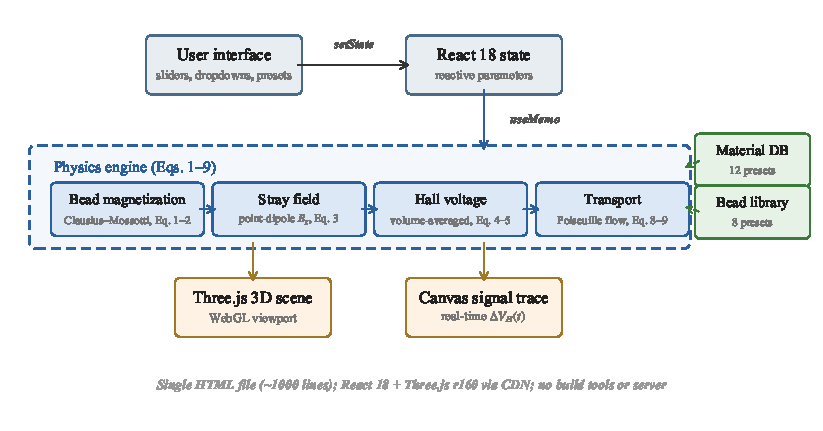
\includegraphics[width=\textwidth]{figures/fig1_architecture.pdf}
\caption{Data-flow architecture of the implementation. A pure-JavaScript physics engine evaluates the model (Eqs.~\eqref{eq:moment}--\eqref{eq:poiseuille}) and feeds the React-managed UI, the Three.js 3D scene, the Canvas signal trace, and a 2D axisymmetric FEM solver that provides an independent magnetostatic check on the analytical dipole model.}
\label{fig:architecture}
\end{figure}

The simulation loop uses adaptive sub-stepping: at each animation frame the step is subdivided into $n_{\text{sub}} = \lceil v_{\max}\,\Delta t_{\text{frame}} / (0.4\, w_{\text{sensor}}) \rceil$ sub-steps, ensuring at least two to three evaluations across the signal peak regardless of bead velocity. A parametric sweep engine evaluates $\Delta V_H$ across user-specified ranges of bead diameter, sensor size, flow velocity, applied field, channel height, bead height, or gate voltage by computing Eqs.~\eqref{eq:moment}--\eqref{eq:vh} directly, with optional multi-material comparison over all 12 presets and CSV export. A batch mode injects up to 50 beads under Poiseuille flow and returns per-bead peak $\Delta V_H$, detection status against a user threshold, and aggregate detection rate, mean, standard deviation, and coefficient of variation. Figure~\ref{fig:screenshot} shows the Simulator page, with the parameter controls, the interactive 3D scene, and the live $\Delta V_H$ trace.

\begin{figure}[!htbp]
\centering
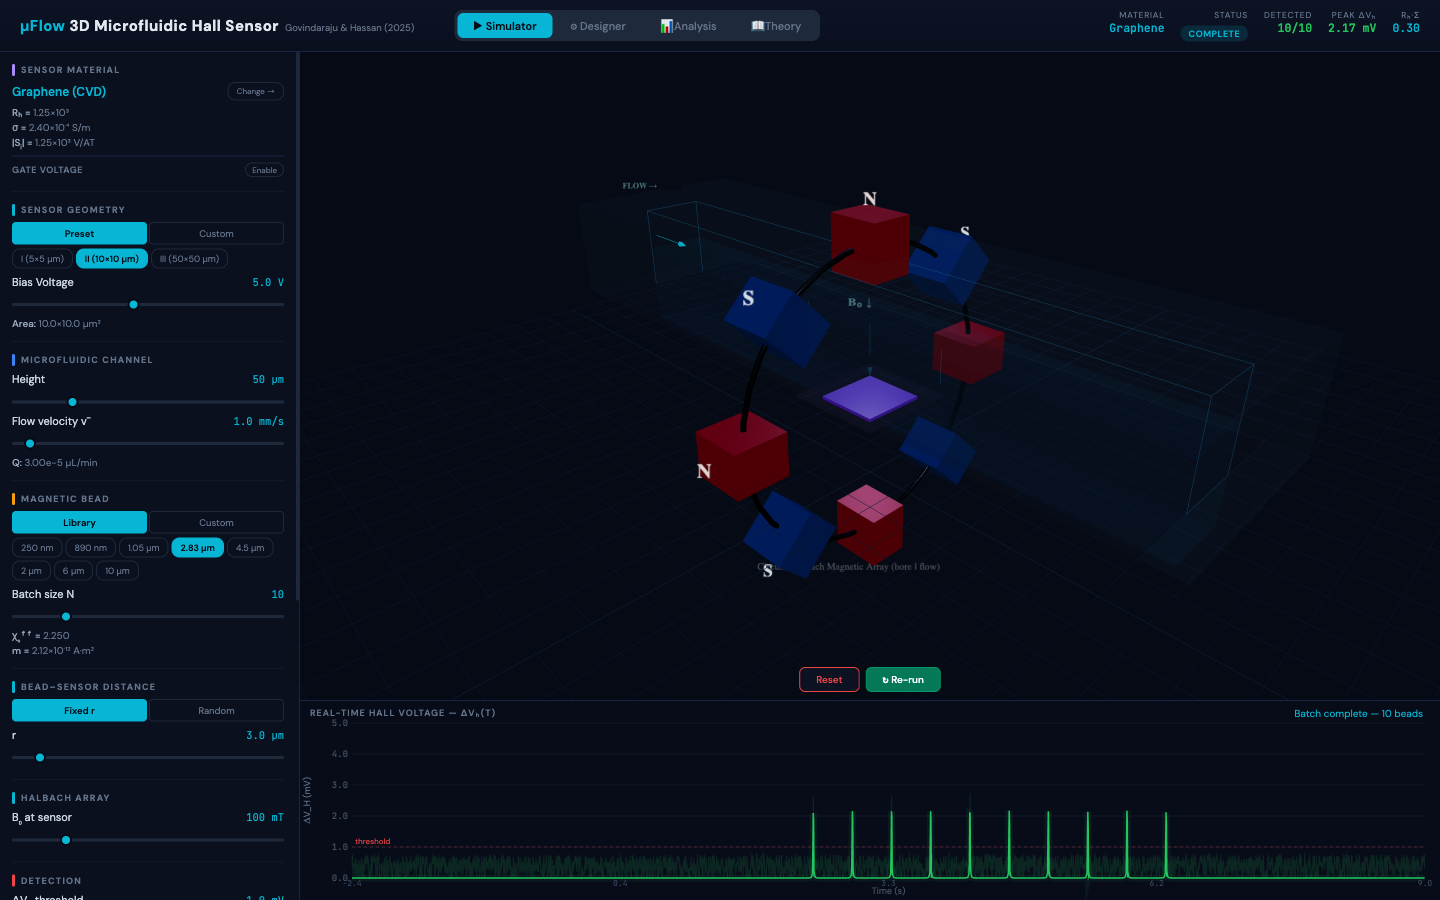
\includegraphics[width=\textwidth]{figures/fig2_screenshot.png}
\caption{Simulator page. Left sidebar: controls for sensor material (with computed $R_H$, $\sigma$, $|S_I|$), geometry, microfluidic channel, and bead selection. Center: 3D viewport showing a bead traversing the Hall sensor within the PDMS microchannel and Halbach array. Bottom: real-time $\Delta V_H$ signal trace (green) with noise-injected overlay and detection threshold (red dashed).}
\label{fig:screenshot}
\end{figure}

\subsection{In-app axisymmetric FEM solver}\label{sec:fem}

The application includes a 2D axisymmetric finite-element magnetostatic solver that validates the point-dipole approximation without external software. The solver computes the perturbation field $\Delta B_z$ from a magnetized bead by solving the magnetic scalar-potential equation $(1/r)\,\partial_r(r\,\mu_r\,\partial_r\varphi) + \partial_z(\mu_r\,\partial_z\varphi) = 0$ on a structured triangular mesh with adaptive refinement near the bead and sensor, using a preconditioned conjugate-gradient method. Four mesh resolutions are available, from ${\sim}3{,}200$ to ${\sim}39{,}200$ elements. The page reports the height-to-radius ratio $h/r_b$ alongside a side-by-side comparison of the FEM and analytical dipole profiles. At $h/r_b > 3$ the two agree within a few percent; at $h/r_b \approx 1$ the deviation widens as finite bead-volume effects become significant, which is the regime the solver is intended to flag.

% =====================================================================
\section{Validation}\label{sec:validation}
% =====================================================================

% ------------------------------------------------------------------------
\subsection{Comparison with FEM-BEM simulations}\label{sec:femvalidation}

We validate the model against the three sensor designs characterized in our companion COMSOL FEM-BEM study \citep{govindaraju2025}. Table~\ref{tab:designs} lists the design parameters and Table~\ref{tab:validation} the validation results. All three designs operate at $h/r_b = 1$, where the bead-center height equals the bead radius.

\begin{table}[!htbp]
\caption{Sensor design configurations from \citet{govindaraju2025}. All use $R_H = 1.25\times10^{-3}$\,m$^3$/C, $\sigma = 1040$\,S/m, $V_{\text{bias}} = 5$\,V, $B_0 = 50$\,mT, magnetite beads ($\mu_r = 10$). The area ratio is $\pi r_b^2/(w\,l)$ with square sensors $l = w$.}
\label{tab:designs}
\centering
\footnotesize
\begin{tabular}{@{}lccc@{}}
\toprule
Parameter & Design~I & Design~II & Design~III \\
\midrule
Sensor width $w$ ($\mu$m) & 5 & 10 & 50 \\
Sensor thickness $t$ ($\mu$m) & 0.5 & 1 & 1 \\
Bead diameter $d_b$ ($\mu$m) & 2 & 6 & 10 \\
Bead-center height $r$ ($\mu$m) & 1 & 3 & 5 \\
Bead-to-sensor area ratio & 0.13 & 0.28 & 0.03 \\
\bottomrule
\end{tabular}
\end{table}

\begin{table}[!htbp]
\caption{Validation of the analytical model against COMSOL FEM-BEM results \citep{govindaraju2025}, bead positioned directly above sensor center. Deviation reported relative to the COMSOL value.}
\label{tab:validation}
\centering
\footnotesize
\begin{tabular}{@{}lcccc@{}}
\toprule
Design & COMSOL (mV) & Model (mV) & Deviation (\%) & Direction \\
\midrule
I ($5\times5$\,$\mu$m) & 21.375 & 16.63 & 22.2 & model below \\
II ($10\times10$\,$\mu$m) & 42.79 & 44.86 & 4.8 & model above \\
III ($50\times50$\,$\mu$m) & 3.056 & 2.58 & 15.6 & model below \\
\bottomrule
\end{tabular}
\end{table}

The analytical model reproduces the COMSOL Hall voltage to within 4.8\% at the favorable bead-to-sensor area ratio of Design~II. At the off-optimum Designs~I and~III the point-dipole approximation deviates by 22\% and 16\%, consistent with its known near-field limit at $h/r_b = 1$. The design-to-design spread is not an $h/r_b$ effect alone, since all three designs sit at $h/r_b = 1$; it is governed by the bead-to-sensor area ratio. Design~II (area ratio 0.28) concentrates the bead's stray-field footprint within the sensor active area, where the dipole approximation captures most of the volume-averaged field. Design~I (area ratio 0.13) under-covers the bead's near field with a small sensor, so the dipole under-estimates the actual field by missing the finite-volume contribution. Design~III (area ratio 0.03) over-averages the bead's field across a large sensor, so the residual near-field error has a larger fractional effect on the small mean. Figure~\ref{fig:validation} presents these results graphically. This pattern, where the dipole approximation is accurate near the area-ratio optimum and degrades away from it, motivates the in-app axisymmetric FEM solver (Section~\ref{sec:fem}) for users working at $h/r_b \lesssim 1.5$.

\begin{figure}[!htbp]
\centering
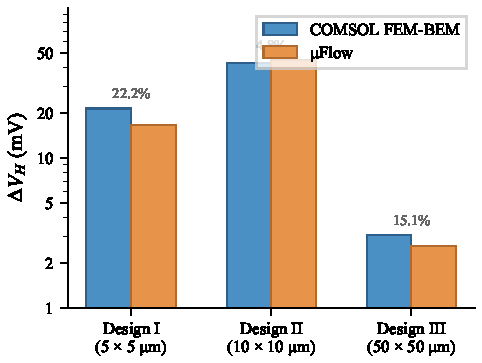
\includegraphics[width=\columnwidth]{figures/fig3_validation.pdf}
\caption{Hall voltage predicted by the analytical model versus COMSOL FEM-BEM \citep{govindaraju2025} for three sensor designs. The model agrees with COMSOL to within 4.8\% at the favorable bead-to-sensor area ratio of Design~II (0.28); at the off-optimum Designs~I and~III the point-dipole approximation deviates by 22\% and 16\%, consistent with its near-field limit at $h/r_b = 1$.}
\label{fig:validation}
\end{figure}

The volume-averaging quadrature is converged at the default resolution. A convergence study at Design~II parameters shows that the $16\times16\times8$ grid gives \SI{44.86}{\milli\volt}, within 0.044\% of a $64\times64\times32$ reference, and the $8\times8\times4$ default deviates by only 0.18\%. The quadrature error is therefore negligible compared with the point-dipole near-field error at $h/r_b = 1$, which dominates the model uncertainty. Combining the dipole near-field contribution, the quadrature contribution, and the ${\pm}\SI{20}{\percent}$ batch-to-batch variation in bead volume fraction $\phi$ \citep{fonnum2005} in quadrature, the total model uncertainty for $\Delta V_H$ is bounded by the deviations in Table~\ref{tab:validation} at $h/r_b = 1$ and falls to a few percent at $h/r_b > 3$.

% ------------------------------------------------------------------------
\subsection{Consistency with published detection experiments}\label{sec:expvalidation}

To assess the full signal chain beyond the COMSOL comparison, we check the model against published microfluidic and micro-Hall bead-detection experiments. Exact quantitative reproduction is limited because the published reports do not always specify the precise bead-sensor distance, bias, and sensor geometry needed to reconstruct the measurement, so we assess order-of-magnitude consistency.

\textit{InAs micro-Hall (low-microvolt regime).} \citet{mihajlovic2005} resolved a single \SI{2.8}{\micro\meter} M-280 Dynabead on an InAs quantum-well micro-Hall cross, measuring a Hall-voltage drop of $\Delta V_H = \SI{2.0}{\micro\volt}$ corresponding to a sensed stray-field change of ${\sim}\SI{80}{\micro\tesla}$. \citet{aledealat2009} extended this InAs platform to a flowing PDMS microchannel and detected \SI{2.6}{\micro\meter} Bangs Laboratories beads in real time in a slow-flow regime (${\sim}\SI{3}{\micro\meter\per\second}$ at \SI{1}{\micro\liter\per\minute}), recording a bipolar Hall transient over seconds-scale transits as a group of about three beads crossed the sensor. Entering the InAs/AlSb 2DEG preset ($S_I = \SI{625}{\volt\per\ampere\per\tesla}$) for an M-280 bead at comparable geometry, the model predicts $\Delta V_H \approx \SI{1.0}{\micro\volt}$, the same order of magnitude as the measured \SIrange{1}{2}{\micro\volt} range, and reproduces the bipolar waveform shape that arises from the $B_z$ sign change at lateral offsets (Eq.~\eqref{eq:dipole}).

\textit{Si CMOS (microtesla field regime).} \citet{besse2002} detected a single M-280 bead with a \SI{2.4}{\micro\meter}$\times$\SI{2.4}{\micro\meter} Si CMOS Hall sensor ($S_I = \SI{175}{\volt\per\ampere\per\tesla}$, $R = \SI{8.5}{\kilo\ohm}$, $I_b = \SI{0.3}{\milli\ampere}$, bead-center distance $r = \SI{7}{\micro\meter}$), reporting magnetic-induction changes of more than \SI{20}{\micro\tesla} under AC excitation with lock-in detection at \SI{520}{\hertz}, against a thermal-noise-limited field resolution of ${\sim}\SI{0.2}{\micro\tesla}/\sqrt{\si{\hertz}}$. The reported signal is a field-induction change of order tens of microtesla driven by their applied AC field, and the model's single-bead stray-field prediction for this configuration is in the same microtesla-to-tens-of-microtesla range. We therefore claim order-of-magnitude consistency at the field level, not reproduction of a specific Hall-voltage magnitude, since their lock-in measurement convolves the bead susceptibility with an externally applied modulation field that the static model does not represent.

\textit{Outside the validated regime.} \citet{gabureac2013} resolved single \SI{1}{\micro\meter} beads with a \SI{500}{\nano\meter} nanocomposite Hall sensor, reporting \SIrange{100}{500}{\nano\volt} signals. For this configuration the bead diameter exceeds the sensor width by $2\times$, the granular nanocomposite transport parameters are underspecified for the present model, and the model prediction (${\sim}\SI{44}{\micro\volt}$) is about two orders of magnitude above the reported signal. This configuration falls outside the model's validated regime, and we report it as such rather than as a successful comparison.

% =====================================================================
\section{Results and design rules}\label{sec:results}
% =====================================================================

This section uses the parametric sweep engine to extract design rules. Unless otherwise noted the default configuration is Design~II ($w = \SI{10}{\micro\meter}$, $t = \SI{1}{\micro\meter}$, $d_b = \SI{6}{\micro\meter}$, $r = \SI{3}{\micro\meter}$, $B_0 = \SI{50}{\milli\tesla}$, $V_{\text{bias}} = \SI{5}{\volt}$).

% ------------------------------------------------------------------------
\subsection{Geometry optimization and the area-ratio optimum}\label{sec:geometry}

Figure~\ref{fig:distance} shows $\Delta V_H$ versus bead-sensor distance $r$ for the three sensor sizes. The $1/r^3$ dipolar decay is evident for all designs. At close range ($r < \SI{2}{\micro\meter}$), the \SI{5}{\micro\meter} sensor produces the strongest signal because its small area concentrates the volume-averaged field; at larger distances ($r > \SI{5}{\micro\meter}$), the \SI{10}{\micro\meter} sensor with a \SI{6}{\micro\meter} bead dominates because the bead's larger moment ($m \propto r_b^3$) compensates for geometric dilution.

\begin{figure}[!htbp]
\centering
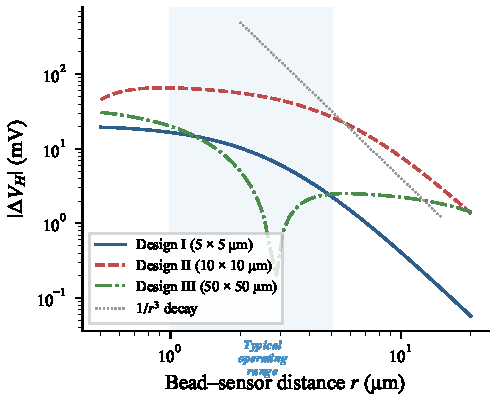
\includegraphics[width=\columnwidth]{figures/fig4_distance.pdf}
\caption{Hall voltage $\Delta V_H$ versus bead-sensor distance for the three validated designs. The $1/r^3$ dipolar decay is evident on the log-log scale. Design~II provides the strongest signal within the typical microfluidic operating range ($r = \SIrange{1}{5}{\micro\meter}$) owing to its favorable bead-to-sensor area ratio.}
\label{fig:distance}
\end{figure}

The sensitivity map in Fig.~\ref{fig:sensitivity} sweeps bead diameter (\SIrange{1}{15}{\micro\meter}) against sensor width (\SIrange{5}{100}{\micro\meter}) and reveals that the maximum $\Delta V_H$ lies along a diagonal corresponding to bead-to-sensor area ratios of 0.1--0.5. The optimum arises from a competition between two scaling laws: the bead moment grows as $m \propto d_b^3$, favoring large beads, while the volume-averaged stray field falls as the sensor area exceeds the bead's field footprint, favoring small sensors. The optimum occurs where the bead's stray-field extent approximately matches the sensor active area.

\begin{figure}[!htbp]
\centering
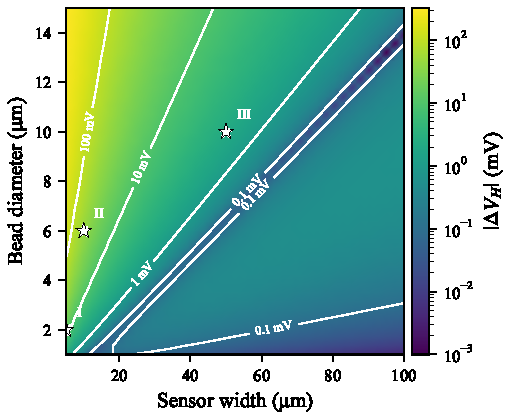
\includegraphics[width=\columnwidth]{figures/fig7_sensitivity.pdf}
\caption{Sensitivity map of $\Delta V_H$ as a function of bead diameter and sensor width ($B_0 = \SI{50}{\milli\tesla}$, $V_{\text{bias}} = \SI{5}{\volt}$). The optimum lies along a diagonal corresponding to bead-to-sensor area ratios of 0.1--0.5, the regime identified by \citet{mihajlovic2007} as noise-optimal, in which the sensor active area is comparable to the bead footprint. Stars mark the three validated designs.}
\label{fig:sensitivity}
\end{figure}

This area-ratio optimum, derived here from the signal magnitude alone, coincides with the regime, identified by \citet{mihajlovic2007} as noise-optimal, in which the sensor active area is comparable to the bead footprint. The two criteria agree from opposite directions, signal and noise, which strengthens the design rule: the sensor width should approximately match the bead diameter. For Dynabeads M-280 ($d_b = \SI{2.8}{\micro\meter}$), the map predicts an optimal sensor width of \SIrange{5}{15}{\micro\meter}; for M-450 ($d_b = \SI{4.5}{\micro\meter}$), \SIrange{8}{25}{\micro\meter}. These match the sensor dimensions used in published single-bead experiments: \citet{mihajlovic2005} used a \SI{5}{\micro\meter} sensor for \SI{2.8}{\micro\meter} M-280 beads, and \citet{kim2014} observed that the planar Hall signal fell when the sensor area exceeded the bead's stray-field footprint.

% ------------------------------------------------------------------------
\subsection{Cross-material signal-to-noise ranking}\label{sec:crossmaterial}

Figure~\ref{fig:materials} compares the 12 material presets under identical Design~II geometry and bead conditions. The $\Delta V_H$ values span nearly three orders of magnitude and track carrier mobility, since $\Delta V_H \propto R_H\, \sigma \propto \mu$ for a given geometry (Eq.~\eqref{eq:vh}). InSb quantum wells and graphene/hBN produce the strongest intrinsic signals; Si CMOS and AlGaN/GaN are among the weakest. CVD graphene on SiO$_2$ offers a practical intermediate that is compatible with wafer-scale integration \citep{shah2023}, while AlGaN/GaN, though weaker, operates reliably above \SI{500}{\kelvin} \citep{zhang2021} where graphene and InSb would degrade.

\begin{figure}[!htbp]
\centering
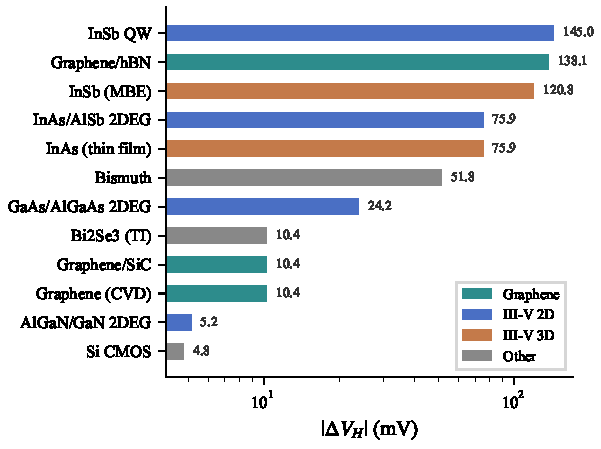
\includegraphics[width=\columnwidth]{figures/fig5_materials.pdf}
\caption{Cross-material comparison of $\Delta V_H$ under identical geometry and bead conditions (Design~II, $B_0 = \SI{50}{\milli\tesla}$, $V_{\text{bias}} = \SI{5}{\volt}$). The Hall voltage tracks carrier mobility; InSb QW and graphene/hBN are strongest, Si CMOS and AlGaN/GaN among the weakest. Bars are color-coded by material family.}
\label{fig:materials}
\end{figure}

The $\Delta V_H$ ranking alone is insufficient for sensor selection because it ignores the material-specific noise floor. Table~\ref{tab:noise} reports $\Delta V_H$, the total noise voltage $V_n$, SNR, and $B_\text{min}$ for five representative platforms at Design~II, computed from Eqs.~\eqref{eq:rsq}--\eqref{eq:snr} with published $\alpha_H$ and mobility values. Across these five, the $\Delta V_H$ ratio between graphene/hBN (\SI{0.39}{\milli\volt}) and Si CMOS (\SI{0.086}{\milli\volt}) is about $4.5\times$, but the SNR ratio is far larger because Si CMOS carries a much higher $1/f$ floor: graphene/hBN reaches SNR ${\sim}2060$ while Si CMOS reaches only ${\sim}12$ at the same geometry. Platforms with low carrier density (high $S_I$) can paradoxically suffer higher $1/f$ noise through the reduced carrier count $N$ in Eq.~\eqref{eq:flicker}, so material selection must be made on SNR rather than $\Delta V_H$ alone. This is the coupled signal-noise comparison that \citet{mihajlovic2007} argued is required for principled platform choice.

\begin{table}[!htbp]
\caption{Cross-material signal and noise at Design~II geometry ($\langle B_z \rangle = \SI{6.90}{\milli\tesla}$, $\Delta f = \SI{1}{\kilo\hertz}$, $T = \SI{300}{\kelvin}$). $V_n$ is the quadrature sum of Johnson--Nyquist and Hooge $1/f$ noise (Eq.~\eqref{eq:snr}).}
\label{tab:noise}
\centering
\footnotesize
\begin{tabular}{@{}lrrrr@{}}
\toprule
Material & $\Delta V_H$ (mV) & $V_n$ (nV) & SNR & $B_\text{min}$ (nT/$\sqrt{\text{Hz}}$) \\
\midrule
Graphene/hBN & 0.392 & 190 & 2060 & 106 \\
InSb QW      & 0.086 & 105 & 820  & 266 \\
CVD graphene & 0.086 & 709 & 122  & 1793 \\
InAs/AlSb    & 0.043 & 159 & 271  & 806 \\
Si CMOS      & 0.086 & 7444 & 12  & 18831 \\
\bottomrule
\end{tabular}
\end{table}

% ------------------------------------------------------------------------
\subsection{Flow-velocity detection window}\label{sec:flowsensitivity}

Flow velocity affects detection through two competing mechanisms: higher velocity raises throughput but shortens the transit time over the sensor, reducing the signal-acquisition window. Figure~\ref{fig:flowrate} shows the detection rate and mean peak $\Delta V_H$ versus mean flow velocity for a batch of 20 beads at Design~II geometry in range mode.

\begin{figure}[!htbp]
\centering
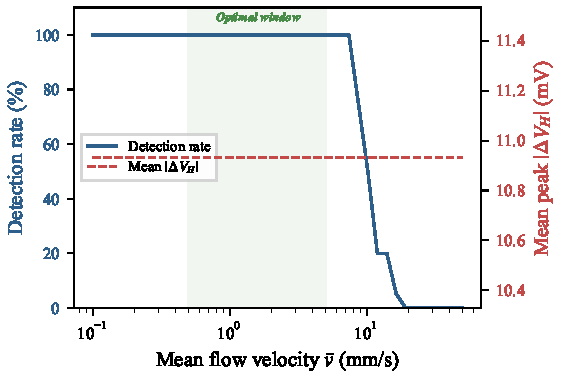
\includegraphics[width=\columnwidth]{figures/fig6_flowrate.pdf}
\caption{Detection rate (left axis) and mean peak $\Delta V_H$ (right axis) versus mean flow velocity for 20 beads at Design~II geometry in range mode. A detection window emerges at $\bar{v} = \SIrange{0.5}{5}{\milli\meter\per\second}$, balancing throughput against adequate signal sampling during bead transit.}
\label{fig:flowrate}
\end{figure}

At low velocities ($\bar{v} < \SI{0.5}{\milli\meter\per\second}$) each bead spends many seconds in the sensing zone, producing well-resolved pulses at low throughput. At moderate velocities ($\bar{v} = \SIrange{0.5}{5}{\milli\meter\per\second}$) the detection rate stays at 100\% and the peak $\Delta V_H$ is governed by bead height rather than velocity, because the adaptive sub-stepping ensures adequate sampling. At high velocities ($\bar{v} > \SI{10}{\milli\meter\per\second}$) the transit time $\tau \approx w/v$ drops below the readout interval and some beads pass the sensor without being captured at peak $\langle B_z \rangle$. This window is consistent with experimental practice: \citet{aledealat2009} operated in a slow-flow regime (${\sim}\SI{3}{\micro\meter\per\second}$ at \SI{1}{\micro\liter\per\minute}), where seconds-scale transits gave well-resolved bipolar Hall pulses. In assay design the high-velocity ceiling balances against throughput: at $\bar{v} = \SI{1}{\milli\meter\per\second}$ in a \SI{50}{\micro\meter} channel the volumetric flow rate is ${\sim}\SI{3}{\nano\liter\per\second}$, sufficient to process ${\sim}\SI{10}{\micro\liter}$ samples in under an hour.

% ------------------------------------------------------------------------
\subsection{Batch detection statistics}\label{sec:batch}

The batch mode injects $N$ beads and records per-bead peak $\Delta V_H$, bead height, and detection status. Table~\ref{tab:batch} shows output for Design~II with 10 beads at fixed height ($r = \SI{3.1}{\micro\meter}$) and in range mode ($r$ uniformly distributed across the channel).

\begin{table}[!htbp]
\caption{Batch detection statistics for Design~II ($w = \SI{10}{\micro\meter}$, $d_b = \SI{6}{\micro\meter}$, $\bar{v} = \SI{1}{\milli\meter\per\second}$, $N = 10$ beads).}
\label{tab:batch}
\centering
\small
\begin{tabular}{lcc}
\toprule
Statistic & Fixed height & Range mode \\
\midrule
Mean peak $\Delta V_H$ (\si{\milli\volt}) & 44.9 & 28.7 \\
Standard deviation (\si{\milli\volt}) & 0.7 & 12.3 \\
Coefficient of variation (\%) & 1.6 & 42.9 \\
Detection rate (\%) & 100 & 90 \\
\bottomrule
\end{tabular}
\end{table}

In fixed-height mode the low coefficient of variation (1.6\%) confirms that signal variation arises solely from numerical discretization. In range mode the CV rises to 42.9\% because beads at different heights experience different stray-field amplitudes through the $1/h^3$ dependence. This is physically realistic: \citet{aledealat2009} observed that the bipolar Hall transient amplitude varied with the bead position in the channel, consistent with the steep height dependence of the dipolar stray field. The 90\% detection rate in range mode reflects beads near the channel ceiling falling below the threshold. Because realistic sedimentation and magnetophoretic drift bias beads toward the floor, this uniform-height result is a conservative lower bound on detection rate.

% =====================================================================
\section{Discussion}\label{sec:discussion}
% =====================================================================

The model substitutes a closed-form evaluation for a volumetric FEM-BEM solve, with speed gained at the cost of accuracy outside its regime of validity. That regime is now quantified.

\textit{Dipole approximation regime.} The model is accurate near the bead-to-sensor area-ratio optimum (0.1--0.5) and at $h/r_b > 3$, where the in-app FEM solver confirms that the point-dipole form recovers the volumetric field to within a few percent (Section~\ref{sec:fem}). At $h/r_b = 1$, the deviation from COMSOL ranges from 4.8\% at the favorable area ratio of Design~II to 22\% and 16\% at the off-optimum area ratios of Designs~I and~III (Table~\ref{tab:validation}). The deviation is a function of how the bead's near field is sampled by the sensor footprint, not of $h/r_b$ alone. For typical microfluidic geometries with \SIrange{1}{5}{\micro\meter} passivation layers and beads in the \SIrange{1}{10}{\micro\meter} range, the operating point lies near the optimum and the model is adequate. Near-contact configurations ($r \to r_b$), relevant to magnetic capture or surface-bound assays, require the multipole corrections that the in-app FEM solver provides and that a full external FEM solve resolves completely.

\textit{Bead magnetization.} The Clausius--Mossotti formulation uses a fixed effective permeability and is accurate below $B_0 \approx \SI{200}{\milli\tesla}$, where composite beads remain in the linear regime. Above this field a Langevin nanoparticle-ensemble model is required. The choice $\mu_r = 10$ for magnetite is consistent with the vibrating-sample-magnetometry fits of \citet{ota2019}.

\textit{Inter-bead coupling and transport.} The model treats each bead independently, valid for the dilute suspensions ($< 10^6$ beads/mL) typical of immunoassay but not for dense magnetic-capture scenarios where bead chains form. The Poiseuille model assumes fully developed laminar flow and neglects entrance effects, bead-wall interactions, and inertial focusing, valid at the low Reynolds numbers ($\text{Re} < 1$) of microfluidic channels below \SI{100}{\micro\meter} in height and below \SI{20}{\milli\meter\per\second} \citep{hewlin2023}.

\textit{Material database.} All parameters are room-temperature values; cryogenic applications require temperature-corrected mobility and carrier density via the custom-material input. The gate-tunable model (Eq.~\eqref{eq:gate}) captures first-order electrostatic gating for 2D materials without quantum-capacitance corrections near charge neutrality.

% =====================================================================
\section{Conclusions}\label{sec:conclusions}
% =====================================================================

We presented a coupled closed-form analytical model of the microfluidic Hall-effect magnetic-bead detection signal chain, comprising Clausius--Mossotti bead magnetization with a volume-fraction correction, a point-dipole stray field, a volume-averaged Hall voltage with geometric correction, Poiseuille transport, and a Johnson--Nyquist/Hooge $1/f$ noise framework, parameterized by a database of 12 sensor platforms. Benchmarked against a companion COMSOL FEM-BEM study, the model reproduces the Hall voltage to within 4.8\% at the favorable bead-to-sensor area ratio of Design~II; at the off-optimum Designs~I and~III the point-dipole approximation deviates by 22\% and 16\%, consistent with its known near-field limit at $h/r_b = 1$. The model is consistent at the order-of-magnitude level with the published InAs micro-Hall single-bead signal of Mihajlovi\'{c} et al.\ and the microtesla field-induction change of Besse et al., and the nanocomposite configuration of Gabureac et al.\ falls outside its validated regime.

The model yields three design rules for microfluidic Hall biosensors. The bead-to-sensor area ratio should lie between 0.1 and 0.5 for maximum $\Delta V_H$, a signal-magnitude optimum that coincides with the regime, identified by \citet{mihajlovic2007} as noise-optimal, in which the sensor active area is comparable to the bead footprint. Detection reliability is maintained at $\bar{v} = \SIrange{0.5}{5}{\milli\meter\per\second}$ for sensors in the \SIrange{5}{50}{\micro\meter} range. Material selection must be made on signal-to-noise rather than $\Delta V_H$ alone, because the Hooge $1/f$ floor reorders the platforms: graphene/hBN and InSb QW lead on both signal and SNR, while Si CMOS, despite a $\Delta V_H$ only about $4.5\times$ below graphene/hBN among the tabulated platforms, falls far behind in SNR through its higher $1/f$ noise. The model is provided as an open browser implementation with an in-app axisymmetric FEM solver that quantifies where the dipole approximation degrades, deployed at \url{https://uflow.studio}.

% =====================================================================
\bmhead{Statements and Declarations}
% =====================================================================

\textbf{Funding.} This work was supported by the National Science Foundation %% TODO: insert NSF award number(s) before submission
and the Department of Electrical and Computer Engineering at Rutgers, The State University of New Jersey.

\textbf{Competing interests.} The authors declare no competing interests.

\textbf{Data availability.} The analytical model is implemented in an open browser application whose source code, build script, and license are available on GitHub at \url{https://github.com/hg293/microfluidic-hall-sensor}, with the running application at \url{https://uflow.studio}. The software is released under the GNU Affero General Public License v3.0 or later (AGPL-3.0-or-later), with trademark, citation, and patent reservations in \texttt{NOTICE.md} at the repository root. An archived snapshot of the version described here will be deposited at Zenodo upon acceptance. No experimental datasets were generated; the simulation outputs reported here are reproducible from the deployed application and are available from the corresponding author on reasonable request, subject to institutional policies.

\textbf{Author contributions.} \textbf{Harshitha Govindaraju:} Conceptualization, Methodology, Software, Validation, Formal analysis, Investigation, Data curation, Visualization, Writing -- original draft, Writing -- review \& editing. \textbf{Umer Hassan:} Conceptualization, Methodology, Supervision, Resources, Funding acquisition, Project administration, Writing -- review \& editing.

\textbf{Use of generative AI.} %% TODO: confirm this names the AI tool(s) you actually used; if AI was used only for copy-editing, Springer does not require declaring it and this line may be removed.
During the preparation of this manuscript the authors used generative AI tools to assist with drafting and editing the text. The authors reviewed and edited all content and take full responsibility for the published article.

% =====================================================================
\bibliography{references}

\end{document}
